\documentclass[11pt,twoside,a4paper]{article}
% http://www-h.eng.cam.ac.uk/help/tpl/textprocessing/latex_maths+pix/node6.html symboles de math
% http://fr.wikibooks.org/wiki/Programmation_LaTeX Programmation latex (wikibook)
%=========================== En-Tete =================================
%--- Insertion de paquetages (optionnel) ---
\usepackage[french]{babel}   % pour dire que le texte est en fran{\'e}ais
\usepackage{a4}				 % pour la taille   
\usepackage[T1]{fontenc}	 % pour les font postscript
%% \usepackage{chancery}
\usepackage{frcursive}
\usepackage{epsfig}			% pour gerer les images
%\usepackage{psfig}
\usepackage{amsmath, amsthm} % tres bon mode mathematique
\usepackage{amsfonts,amssymb}% permet la definition des ensembles
\usepackage{float}		 	% pour le placement des figure
\usepackage{verbatim}

\usepackage{longtable} % pour les tableaux de plusieurs pages

\usepackage[table]{xcolor} % couleur de fond des cellules de tableaux

\usepackage{lastpage}

\usepackage{multirow}

\usepackage{multicol} % pour {\'e}crire dans certaines zones en colonnes : \begin{multicols}{nb colonnes}...\end{multicols} 

% \usepackage[top=1.5cm, bottom=1.5cm, left=1.5cm, right=1.5cm]{geometry}
% gauche, haut, droite, bas, entete, ente2txt, pied, txt2pied
\usepackage{vmargin}
\setmarginsrb{1.00cm}{1.00cm}{1.00cm}{1.00cm}{15pt}{3pt}{50pt}{20pt}

\usepackage{lscape} % changement orientation page
%\usepackage{frbib} % enlever pour obtenir references en anglais
% --- style de page (pour les en-tete) ---
\pagestyle{empty}

\def\txtTITLE{Conspiration : Mode d'emploi} %%%%% !! TITRE !! %%%%%
\def\imgCORNER{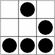
\includegraphics[width=0.25cm]{../../../../../imgGraphics/logos/glider/logo-glider.png}}

%--- Definitions de nouvelles couleurs ---
\definecolor{verylightgrey}{rgb}{0.8,0.8,0.8}
\definecolor{verylightgray}{gray}{0.80}
\definecolor{lightgrey}{rgb}{0.6,0.6,0.6}
\definecolor{lightgray}{gray}{0.6}



% % % en-tete et pieds de page configurables : fancyhdr.sty

% http://www.trustonme.net/didactels/250.html

% http://ww3.ac-poitiers.fr/math/tex/pratique/entete/entete.htm
% http://www.ctan.org/tex-archive/macros/latex/contrib/fancyhdr/fancyhdr.pdf
\usepackage{fancyhdr}
\pagestyle{fancy}
% \newcommand{\chaptermark}[1]{\markboth{#1}{}}
% \newcommand{\sectionmark}[1]{\markright{\thesection\ #1}}
\fancyhf{}
\fancyhead[LE,RO]{\bfseries\thepage}
\fancyhead[LO]{\bfseries\rightmark}
\fancyhead[RE]{\bfseries\leftmark}
\fancyfoot[LE]{\thepage /\pageref{LastPage} \hfill
	\scriptsize{\txtTITLE} % TITLE
\hfill \imgCORNER }
\fancyfoot[RO]{\imgCORNER \hfill
	\scriptsize{\txtTITLE} % TITLE
\hfill \thepage /\pageref{LastPage}}
\renewcommand{\headrulewidth}{0.5pt}
\renewcommand{\footrulewidth}{0.5pt}
\addtolength{\headheight}{0.5pt}
% \fancypagestyle{plain}{
	% \fancyhead{}
	% \renewcommand{\headrulewidth}{0pt}
% }

\usepackage{lettrine}
\usepackage{fancybox}

\title{\txtTITLE}
\date{ --- }

%============================= Corps =================================
\begin{document}

\setlength\parindent{0pt} % \noindent for all document

~\\

\vfill

\begin{center}
	\textbf{\Huge \txtTITLE}
\end{center}

\vfill

%% \tableofcontents

\begin{center}
	\textbf{\Huge INSPIREZ, CONSPIREZ !~\\ LA CONSPIRATION : MODE D'EMPLOI}
\end{center}

\textbf{\scriptsize {\`A} l'heure du retour d'\emph{Aux fronti{\`e}res} du r{\'e}el sur nos petits {\'e}crans et de la sortie annonc{\'e}e de Dossiers X (la V. F. du jeu \emph{Conspiracy X}), peut-{\^e}tre est-il temps de se poser les vraies questions : qui nous gouverne ? Sont-ils d{\'e}j{\`a} parmi nous ? C'est le moment de faire trembler vos joueurs en leur d{\'e}montrant qu'un univers de jeu de r{\^o}le peut-{\^e}tre aussi fou que le monde r{\'e}el... }~\\
\texttt{\scriptsize (Originellement Publi{\'e} dans : Casus Belli num{\'e}ro 98 (octobre 1996, Excelsior Publications) pages 24 {\`a} 28. }~\\ 

\vfill

\clearpage

\begin{multicols*}{2}

\textbf{\Large TH{\'E}ORIE}~\\

\textbf{\large DE QUOI PARLE-T-ON ?}~\\

La notion de conspiration, dans l'acceptation la plus large du terme, est sans doute aussi ancienne que celle de civilisation. Pour le dictionnaire, assez r{\'e}serv{\'e} sur le sujet, une conspiration est <<une machination tram{\'e}e contre une personne ou une institution, le plus souvent un r{\'e}gime politique>>. Dans le cadre d'un jeu de r{\^o}le, on pr{\'e}f{\`e}rera parler d'une manoeuvre secr{\`e}te de grande envergure, destin{\'e}e soit {\`a} conf{\'e}rer {\`a} ses instigateurs un certain pouvoir sur tout ou partie du monde, soit {\`a} occulter des informations ou {\`a} conduire des exp{\'e}rimentations illicites. La diff{\'e}rence entre ces deux notions est fondamentale : g{\'e}n{\'e}ralement, on a affaire dans le premier cas {\`a} des soci{\'e}t{\'e}s secr{\`e}tes et dans le second... au gouvernement, vieux fantasme r{\'e}current sur lequel surfent actuellement les cr{\'e}ateurs d'Aux fronti{\`e}res du r{\'e}el. Attention aux confusions : le scandale du sang contamin{\'e} en France, par exemple, peut difficilement {\^e}tre consid{\'e}r{\'e} comme une conspiration. Il s'agit d'une n{\'e}gligence criminelle, mais ne r{\'e}sultant en aucun cas d'une action concert{\'e}e, planifi{\'e}e et orchestr{\'e}e dans quelque but occulte (m{\^e}me s'il y aura toujours des parano{\"i}aques pour vous dire le contraire). ~\\

\textbf{\large LE FOND DU PROBL{\`E}ME}~\\
En ces temps pr{\'e}tendument modernes, o{\`u} la mondialisation de l'information est cens{\'e}e apporter au citoyen connaissance et ma{\^i}trise de l'environnement sociopolitique, o{\`u} les syst{\`e}mes de contr{\^o}le r{\'e}ciproque (qui la base de la Constitution am{\'e}ricaine) et la solidit{\'e} des institutions d{\'e}mocratiques sont cens{\'e}es garantir une certaine id{\'e}e de la morale et de la justice, l'homme d{\'e}couvre avec stup{\'e}faction que rien n'a chang{\'e} : sa t{\'e}l{\'e}vision lui ment, son gouvernement lui cache des choses, ses tribunaux sont corrompus, etc. Les m{\'e}dias, toujours mieux inform{\'e}s, se font les t{\'e}moins de cette d{\'e}liquescence – alors que la corruption, la tricherie et le mensonge ont toujours fait partie de la r{\'e}alit{\'e} politique de ce monde, dans l'Ath{\`e}nes de Platon comme {\`a} Washington. L'homme moderne se d{\'e}couvre soudain fragile, vuln{\'e}rable, soumis aux machinations d'un gouvernement qu'il a sans doute contribu{\'e} {\`a} amener au pouvoir. Cette perspective est d'autant plus effrayante qu'elle s'inscrit dans un processus g{\'e}n{\'e}ralis{\'e} : le SIDA vous interdit de faire l'amour en toute tranquillit{\'e}, la maladie de Kreutzfeld-Jacob vous emp{\^e}che de profiter d'un bon steak et votre gouvernement vous poignarde dans le dos, quand il n'est pas tout simplement verrouill{\'e} par des institutions qu'il se r{\'e}v{\`e}le incapable de contr{\^o}ler : la trahison se d{\'e}mocratise et la rumeur gagne du terrain. ~\\
Les th{\'e}ories conspirationnistes jouent avec ces peurs comme la t{\'e}l{\'e}vision avec la solitude des spectateurs. On dira <<th{\'e}ories>> parce qu'{\`a} l'exception de quelques faits publiquement av{\'e}r{\'e}s, rien n'a jamais {\'e}t{\'e} prouv{\'e} (Roswell / JFK, m{\^e}me combat !). Si les explications propos{\'e}es d{\'e}montrent une chose, c'est bien le besoin de leurs inventeurs de se faire peur et de remettre en question le fonctionnement des institutions contemporaines, intention {\`a} priori louable quand elle ne tourne pas au d{\'e}lire de pers{\'e}cution. ~\\

\textbf{\large LA SPIRALE PARANO{\"I}AQUE}~\\
Le moteur essentiel des th{\'e}ories conspirationnistes reste la parano{\"i}a. La plupart fonctionnent en effet sur un raisonnement logique assez pervers : vous n'y croyez pas ? Parfait : c'est ce qu'ILS veulent. Une {\'e}mission a d{\'e}montr{\'e} le contraire ? Mais qui a produit cette {\'e}mission ? EUX, sans aucun doute (remplacez <<eux>> par l'entit{\'e} de votre choix : nazis, FBI, extra-terrestres, gouvernement ou mieux encore, tout \c{c}a m{\'e}lang{\'e}). Impossible de rassurer un type qui croit vraiment {\`a} \c{c}a, si vous insistez trop, il finira par penser que vous {\^e}tes de LEUR c{\^o}t{\'e}. Certains Am{\'e}ricains estiment qu'Ind{\'e}pendance Day est un film de propagande mis au point par l'arm{\'e}e am{\'e}ricaine pour tourner le th{\`e}me de Roswell en d{\'e}rision, sur le th{\`e}me <<vous voyez bien que \c{c}a ne peut pas {\^e}tre vrai, puisque c'est dans un film>>. Le probl{\`e}me de cette th{\'e}orie, c'est que la plupart des Am{\'e}ricains ont plut{\^o}t tendance {\`a} penser que c'est justement vrai parce que c'est dans un film : bonjour le cercle vicieux... ~\\
Pour un vrai parano{\"i}aque, rien n'est jamais vraiment s{\^u}r. Les conspirationnistes ont {\'e}t{\'e} d{\'e}masqu{\'e}s ? Il s'agit certainement d'une conspiration. Et ainsi de suite... ~\\

\begin{center} \rule{0.45\textwidth}{0.01cm} \end{center}
%% \vfill
%% \columnbreak

\textbf{\Large EXEMPLE}~\\

\textbf{\large LUTHER KING, OU LA R{\'E}ALIT{\'E} VAINQUEUR PAR K.O.}~\\
Si l'assassinat de John Fitzgerald Kennedy est rest{\'e} dans toutes les m{\'e}moires (et continue d'alimenter les fantasmes de la plupart des amateurs de conspiration), celui de Martin Luther King reste au moins aussi spectaculaire, compliqu{\'e} et riche d'implications que le <<complot>> de Dallas. D{\'e}sinformation, coups bas et manipulations pr{\'e}sum{\'e}es, tous les {\'e}l{\'e}ments sont r{\'e}unis pour faire de cette affaire l'une des {\'e}nigmes les plus explosives de notre temps. Vingt-huit an apr{\`e}s, [en 1996] la th{\'e}orie conspirationniste est plus vivace que jamais. {\`A} vous de recoller les morceaux... ~\\

\vfill
\columnbreak

\textbf{\large \emph{CIA} ? \emph{FBI} ? \emph{KKK} ? }~\\
Les faits, tout d'abord. Apr{\`e}s qu'une manifestation initi{\'e}e par Luther King {\`a} Memphis ait tourn{\'e} au drame, le pasteur se retire au Holiday Inn local pour panser ses blessures. La presse locale joue les grandes dames scandalis{\'e}es et reproche au leader noir d'avoir choisi un h{\^o}tel tenu par des Blancs. Piqu{\'e} au vif, King part d'installer au Motel Lorraine, comme le lui ont sugg{\'e}r{\'e} certains {\'e}ditorialistes, que l'on accusera plus tard d'avoir {\'e}t{\'e} manipul{\'e}s par le FBI. C'est sur le balcon de sa chambre, dans ce m{\^e}me motel, que King sera abattu d'une balle en plein c\oe ur, apr{\`e}s avoir {\'e}voqu{\'e} la possibilit{\'e} de sa mort quelques heures auparavant. L'un des gardes du corps pointe aussit{\^o}t le doigt vers une fen{\^e}tre de l'immeuble d'en face, et tous les regards se tournent dans la direction indiqu{\'e}e. Effectivement, un homme sort en courant du b{\^a}timent en question et prend la fuite {\`a} bord d'une mustang blanche, non sans avoir abandonn{\'e} derri{\`e}re lui un sac contenant un fusil des effets personnels. Le <<criminel>> James Earl Ray, sera finalement rattrap{\'e} deux mois plus tard {\`a} Londres. Les enqu{\^e}teurs du FBI, d'abord {\'e}trangement muets sur son identit{\'e}, se r{\'e}v{\`e}lent finalement incapable de trouver une quelconque explication {\`a} son geste et d{\'e}cident en d{\'e}sespoir de cause que Ray <<d{\'e}testait les Noirs>>. Le premier avocat de Ray lui conseille de plaider coupable pour {\'e}chapper {\`a} la peine de mort... et {\'e}viter une enqu{\^e}te approfondie, ajouterons certains. 
Mais un second avocat refuse de jouer le jeu : mis en confiance, Ray affirme qu'il n'a pas tu{\'e} MLK, mais qu'il {\'e}tait pr{\'e}sent le jour du meurtre, et qu'il a {\'e}t{\'e} trahi par un homme nomm{\'e} <<Raoul>>, l'un des pseudonymes choisis par un certain Jules Ricco Kimble – Dangereux criminel poss{\'e}dant notamment des connexions avec le Klu Klux Klan. Interrog{\'e} {\`a} son tour, Kimble que Ray <<n'{\'e}tait qu'un pion>>, et que les v{\'e}ritables assassins {\'e}taient en r{\'e}alit{\'e} des hommes de la CIA. Une seule personne peut contredire son t{\'e}moignage : Charles Stephens, qui d{\'e}clare avoir vu Ray descendre de l'immeuble, un fusil {\`a} la main. D'autres t{\'e}moins affirment cependant que Stephens {\'e}tait compl{\`e}tement saoul au moment du drame, et m{\^e}me sa propre {\'e}pouse r{\'e}fute son t{\'e}moignage. L'homme en question, jure-t-elle, n'{\'e}tait pas James Ray. Au final, ce seront les affirmations de Stephens, et elles seules, qui seront pourtant prises en compte. Grace Stephens, quant {\`a} elle, sera rapidement plac{\'e}e en h{\^o}pital psychiatrique. Contre son gr{\'e}, bien entendu. 

\begin{center} \begin{minipage}[ht]{0.30\textwidth}
	\emph{Le texte que vous {\^e}tes en train de lire fait partie d'une gigantesque conspiration. Lorsque vous l'aurez parcouru, vous penserez que ce genre de sujet {\`a} tout juste bon {\`a} amuser les r{\^o}listes. Mais savez-vous qui {\'e}crit vraiment dans Casus Belli ?}~\\
\end{minipage} \end{center}

\textbf{\textit{\large Hallucinant ?}}~\\
L'histoire est pourtant loin d'{\^e}tre finie. Avant d'{\^e}tre rattrap{\'e} par le FBI, James Ray avait eu le temps de passer de Memphis {\`a} Londres, via Toronto et le Portugal. Les faux passeports dont il {\'e}tait muni (lesquels, d'apr{\`e}s Kimble, lui avaient {\'e}t{\'e} fournis par la CIA elle-m{\^e}me) correspondaient {\`a} des personnes r{\'e}elles, de la m{\^e}me morphologie et du m{\^e}me {\^a}ge que Ray. Ce dernier affirma avoir consult{\'e} un registre de naissance pour s'en inspirer. Fait curieux cependant, la signature de l'un des passeports correspondait {\`a} la signature r{\'e}elle de l'alias en question, ce qui tendait {\`a} prouver que Ray s'{\'e}tait procur{\'e} la v{\'e}ritable signature. Autre fait troublant : le second avocat de James Ray affirmait que l'un des gardes du corps de MLK, celui qui avait si promptement point{\'e} le doigt vers la fen{\^e}tre de James Ray, {\'e}tait en r{\'e}alit{\'e} un membre de la police locale, et l'un des fauteurs de trouble qui avait transform{\'e} la manifestation de Memphis en {\'e}meute. Agent double ? Il est int{\'e}ressant de noter que le chef du FBI de l'{\'e}poque, J. Edgar Hoover, tenait Martin Luther King pour l'homme le plus dangereux des Etats-Unis, et pour un individu <<d{\'e}g{\'e}n{\'e}r{\'e}>>. On racontait {\`a} l'{\'e}poque que le FBI avait d{\'e}j{\`a} essay{\'e} de pousser MLK au suicide en exer\c{c}ant des chantages sur sa vie priv{\'e}e. Fait {\'e}tonnant, l'homme charg{\'e} de cette <<mission>> {\'e}tait {\'e}galement responsable de l'enqu{\^e}te qui d{\'e}signa James Earl Ray comme coupable du meurtre...

\vfill

\textbf{\textit{\large Pour quelques notes de plus : }}
\begin{itemize}
	\item[$\bullet$] L'un  des gros bonnets de la p{\`e}gre de Chicago (Sam Giancana) aurait, selon son chauffeur, refus{\'e} une offre d'un million de dollars par le FBI pour assassiner Luther King en r{\'e}torquant : <<Pas question, pas apr{\`e}s que vous ayez g{\^a}ch{\'e} notre accord sur Kennedy de cette fa\c{c}on.>> 
	\item[$\bullet$] De nombreux t{\'e}moins insist{\`e}rent que le fait qu'au moment du meurtre, ce n'{\'e}tait pas une, mais bien deux mustangs blanches qui {\'e}taient gar{\'e}es dans la rue principale devant l'h{\^o}tel. 
	\item[$\bullet$] La pi{\`e}ce que Ray avait lou{\'e}e pour perp{\'e}trer son acte se trouvait dans une annexe au b{\^a}timent principal, en face du balcon de MLK. Ray n'aurait jamais pu l'apprendre de lui-m{\^e}me avant d'avoir lou{\'e} la chambre en question. Qui l'a renseign{\'e} ?
	\item[$\bullet$] Un homme portant le m{\^e}me costume que James Ray fut aper\c{c}u quelques minutes avant le meurtre, dans le restaurant situ{\'e} juste en dessous de la pi{\`e}ce lou{\'e}e par Ray. Il est possible qu'il s'agisse de l'homme qui prit plus tard la fuite... {\`a} bord d'une mustang blanche, emmenant les policiers sur une mauvaise piste, le temps que James Ray puisse s'{\'e}chapper...
\end{itemize}

\begin{center} \rule{0.45\textwidth}{0.01cm} \end{center}

\textbf{\Large PRATIQUE}~\\

\textbf{\large PETIT GUIDE DE LA CONSPIRATION}~\\
Pour {\^e}tre efficace dans un sc{\'e}nario de jeu de r{\^o}le, une conspiration moderne se doit de r{\'e}unir certains {\'e}l{\'e}ments essentiels : 
\begin{itemize}
	\item[$\bullet$] Un <<projet>> hallucinant. Pourquoi se contenter de propager la peste en Afrique ? Autant {\'e}tendre l'{\'e}pid{\'e}mie au monde entier ! Plus cela vous para{\^i}t monstrueux, mieux c'est, du moment que ce n'est pas totalement irr{\'e}alisable ou grotesque (pensez aux grands m{\'e}chants de James Bond). 
	\item[$\bullet$] Une organisation <<{\`a} tiroirs>>. C'{\'e}tait notamment le syst{\`e}me utilis{\'e} par la Golden Dawn de l'Angleterre victorienne. Car si tout le monde est au courant du v{\'e}ritable but du groupuscule, de la soci{\'e}t{\'e} secr{\`e}te ou du gouvernement, il suffit qu'une seule personne parle pour que le projet dans son ensemble soit menac{\'e}. Aussi, dans la plupart des soci{\'e}t{\'e}s secr{\`e}tes, il existe plusieurs rangs d'initi{\'e}s : seuls ceux qui se trouvent en haut de l'{\'e}chelle connaissent les v{\'e}ritables motivations de l'organisation. Les autres croient les conna{\^i}tre. {\'E}videmment, on ne peut {\^e}tre jamais s{\^u}r qu'il n'y a pas quelqu'un au-dessus de soi...
	\item[$\bullet$] Un m{\'e}pris total de l'humanit{\'e}. Les gens normaux ne sont que des pions ou des cobayes de laboratoire. Pourquoi s'en faire pour eux ? Ils mourront bien un jour, de toute fa\c{c}on. Les extraterrestres les consid{\`e}rent comme du b{\'e}tail et la CIA comme de sinistres cr{\'e}tins, jusqu'au jour o{\`u} l'un d'entre eux finit par faire {\'e}chouer leurs plans. 
	\item[$\bullet$] Un service de renseignement insistant et (souvent) maladroit. Cas typique : les fameux Men In Black (Hommes En Noir). La plupart des Am{\'e}ricains ayant {\'e}t{\'e} t{\'e}moins d'apparitions d'OVNI d{\'e}clarent avoir re\c{c}u peu de temps apr{\`e}s l'incident la visite de gorilles patibulaires leur intimant l'ordre de la boucler une fois pour toutes. La fonction de ces hommes, comme on le voit dans Aux fronti{\`e}res du r{\'e}el, est surtout de renforcer la parano{\"i}a des t{\'e}moins en question et de les conforter dans leur certitude. 
	\item[$\bullet$] Un projet {\`a} long terme. Qui dont <<monstrueux>> dit long, tortueux et difficile {\`a} mettre en \oe uvre. Le Grand Plan des Templiers est en pr{\'e}paration depuis pas mal de si{\`e}cles. Enfin, c'est ce qui se dit. 
	\item[$\bullet$] Une <<fausse>> fin. La conspiration Alpha a {\'e}t{\'e} d{\'e}masqu{\'e}e ? Il s'agit d'un proc{\'e}d{\'e} classique destin{\'e} {\`a} attirer l'attention sur une conspiration factice jouant le r{\^o}le de leurre. Tout le monde est bien content que les espions X et Y aient finalement {\'e}t{\'e} arr{\^e}t{\'e}s : ce que tout le monde ignore, c'est qu'ils l'ont fait expr{\`e}s. 
	\item[$\bullet$] Une bonne conspiration doit contenir au moins l'un des {\'e}l{\'e}ments suivants ; les nazis, les extraterrestres, le FBI, la CIA ou tout autre organisme {\'e}quivalent, l'arm{\'e}e et ses bases secr{\`e}tes dans le d{\'e}sert, les exp{\'e}riences m{\'e}dicales, les drogues (le LSD aurait {\'e}t{\'e} introduit aux Etats-Unis sur ordre de la CIA, le SIDA serait le r{\'e}sultat d'une malheureuse exp{\'e}rience de laboratoire), les clones (personne vue {\`a} plusieurs endroits en m{\^e}me temps, comme Lee Harvey Oswald), les morts inexpliqu{\'e}es (quand il s'agit de vraies morts : saviez-vous que Jim Morrisson {\'e}tait toujours vivant ?), le programme spatial (nous ne sommes jamais all{\'e} sur la Lune ; il y a quelque chose sur la face cach{\'e}e de Mars, etc.) et bien s{\^u}r, un pr{\'e}sident cr{\'e}dule, style Jimmy Carter. 
\end{itemize}
 
\begin{center} \rule{0.45\textwidth}{0.01cm} \end{center}
%% \vfill
%% \columnbreak

\textbf{\large ET QU'EST-CE QUE JE FAIT DE TOUT \c{C}A ?}~\\
Une fois que vous aurez mis sur pied une conspiration suffisamment diabolique et perverse, il sera toujours temps de vous poser LA question : de quel c{\^o}t{\'e} se trouvent les personnages de joueurs ? Dans un univers contemporain, il para{\^i}t difficile, {\`a} moins d'avoir une attirance d{\'e}finitive pour le mal, de faire partie des conspirateurs : l'exp{\'e}rience montre qu'ils ne sont gu{\`e}res sympathiques, et qu'ils retombent rarement sur leurs pattes : la CIA fait des aveux publics, Nixon deviens le pr{\'e}sident le plus ha{\"i} de toute l'histoire am{\'e}ricaine, et les Templiers attendent toujours d'{\^e}tre ma{\^i}tres du monde. S'il s'agit de combattre ou de renverser un syst{\`e}me totalitaire, les choses sont bien s{\^u}res diff{\'e}rentes. La cas se rencontre plus souvent dans les jeux m{\'e}di{\'e}vaux-fantastiques ou dans les productions space op{\'e}ra : quoi que de plus excitant que de monter une cabale pour renverser le roi-sorcier du coin et sa cour de mort-vivants putrides ? On parlera alors de conspiration l{\'e}gitime. Cas particulier : la conspiration anti-conspiration, comme dans les dossiers X : les extra-terrestres envahissent la plan{\`e}te avec l'aide d'une poign{\'e}e d'humains, et leurs adversaires rentrent dans la clandestinit{\'e} pour faire {\'e}chouer la man\oe uvre... ~\\
Pour finir, allez donc jeter un \oe il aux documents (authentiques) que nous soumettons {\`a} votre sagacit{\'e} page suivante... et {\`a} vous de jouer  ! ~\\

\textbf{Fabrice Colin}~\\ %% (Illustrations d'origines : Ludovic Debeurme)}~\\

\vfill
\columnbreak

\begin{center} \rule{0.45\textwidth}{0.01cm} \end{center}
 
\textbf{\large DES TH{\'E}ORIES CONSPIRATIONNISTES}~\\
Il existe des centaines de th{\'e}ories conspirationnistes. Certaines sont cr{\'e}dibles, d'autres rel{\`e}vent de la psychiatrie pure et simple et combinent trop d'{\'e}l{\'e}ments d{\'e}lirants pour pouvoir se targuer d'une quelconque cr{\'e}dibilit{\'e} : 
\begin{itemize}
	\item la connexion entre les meurtres de John Fitzgerald Kennedy et de Martin Luther King ; 
	\item les collaborations Nazis / CIA (innombrables versions sur ce th{\`e}me) ; 
	\item le meurtre de JFK en tant que rite ma\c{c}onnique ; 
	\item les connexions Hitler / extraterrestres / soci{\'e}t{\'e}s secr{\`e}tes / royaume de Thul{\'e} (voyez le premier et le troisi{\`e}me Indiana Jones) ; 
	\item les soucoupes volantes stock{\'e}es et utilis{\'e}es comme prototypes par l'arm{\'e}e am{\'e}ricaine depuis les ann{\'e}es 50 ; 
	\item Lee Harvey Oswald, Charles Manson, Mark Davis Chapman (assassin de John Lennon) et la plupart des grands assassins de ce si{\`e}cle [le XX{\`e}me] comme membres de la m{\^e}me secte.
\end{itemize} 
Reportez-vous au paragraphe <<Luther King, ou la r{\'e}alit{\'e} vainqueur par K.O.>>, pour un exemple de conspiration pr{\'e}sum{\'e}e r{\'e}elle. 

\begin{center} \rule{0.45\textwidth}{0.01cm} \end{center}

\textbf{\large INSPI -- CONSPI}~\\
Quelques sources d'inspiration : la collection \emph{Aventures myst{\'e}rieuses} chez J'ai Lu peut fournir de bonnes bases pour des conspirations type \emph{Nephilim}, tout comme le rayon {\'e}sot{\'e}risme des librairies. Les ouvrages sp{\'e}cifiquement centr{\'e}es sur les grandes conspirations sont g{\'e}n{\'e}ralement am{\'e}ricains (exception : l'\emph{{\'E}nigme sacr{\'e}e}, chez Pygmalion). La plupart des auteurs am{\'e}ricains des ann{\'e}es 60-70, de Ginsberg {\`a} Thompson en passant par K. Dick ou Burroughs, sont d'ailleurs de grands paranos devant l'{\'E}ternel. ~\\
Autre piste : \emph{Big book of conspiracies} (chez DC), qui a le m{\'e}rite d'{\^e}tre pr{\'e}sent{\'e} sous forme de BD : marrant et agr{\'e}able {\`a} lire, et commandable dans toute bonne boutique de comics. C{\^o}t{\'e} film, les r{\'e}f{\'e}rences sont innombrables, y compris chez les Fran\c{c}ais. ~\\
Pierre Rosenthal me souffle deux r{\'e}f{\'e}rences {\`a} l'oreille : \emph{Agent trouble} et \emph{Ville {\`a} vendre}, de Jean-Michel Mocky. Les mois {\`a} venir devraient voir grossir la liste de fa\c{c}on effarante, avec notamment \emph{Men In Black} et \emph{X-Files : le film}. ~\\

\begin{center} \rule{0.45\textwidth}{0.01cm} \end{center}

\vfill
\columnbreak

\vfill

\textbf{\Large UNE CONSPIRATION : ~\\une description et une lettre...}~\\

\textbf{\Large OP{\'E}RATION FALLEN ANGELS}~\\

Avec la multiplication des signaux d'origine extra-terrestre capt{\'e}s par les radiot{\'e}lescopes fran\c{c}ais et am{\'e}ricains depuis une trentaine d'ann{\'e}es, les gouvernements ont pris conscience de l'imminence d'un contact avec une forme de vie extraterrestre. Dans l'{\'e}tat actuel des choses, il leur est impossible de savoir sur quel type de relation cette rencontre peut d{\'e}boucher. Il leur faut donc se parer {\`a} toute {\'e}ventualit{\'e}. ~\\

Le 12 octobre 1994, les repr{\'e}sentants des arm{\'e}es fran\c{c}aises, anglaises et am{\'e}ricaines, signent un accord secret pour autoriser la production en s{\'e}rie de cr{\'e}atures clon{\'e}es baptis{\'e}es <<Tasmans>> et parachut{\'e}es au hasard dans le monde entier. ~\\

Les premiers exemplaires de ces cr{\'e}atures sont sortis des laboratoires en f{\'e}vrier 95. Leur r{\^o}le ? R{\'e}pandre dans le monde entier une psychose mill{\'e}nariste contr{\^o}l{\'e}e (syst{\`e}me de surveillance des t{\'e}moins, puce {\'e}lectronique de rep{\'e}rage pour localiser les sp{\'e}cimens) qui culminera en 1999 avec une multiplication du nombre d'apparitions. ~\\

Le but ? {\'E}tudier les r{\'e}percussions d'une d{\'e}couverte de forme de vie extra-terrestre sur les populations (et accessoirement, justifier un programme d'armement biologique des pays concern{\'e}s). On sait le vent de panique qu'avait provoqu{\'e} en son temps Orson Welles en annon\c{c}ant {\`a} la radio une invasion extraterrestre sur les Etats-Unis. Soucieux d'{\'e}viter tout mouvement similaire en cas d'invasion r{\'e}elle, les {\'e}tats-majors des trois pays concern{\'e}s pensent que cette p{\'e}riode agit{\'e}e, troubl{\'e}e par les psychoses pr{\'e}-mill{\'e}naristes et la multiplication d'apparitions d'OVNI est le meilleur moment pour mener {\`a} son terme une exp{\'e}rience de simulation. ~\\

Tout cela ne va pas bien s{\^u}r sans quelques accrocs. Lorsqu'une personne trop proche de l'organisation risque par inadvertance d'enrayer le belle m{\'e}canique, l'exp{\'e}rience se poursuit sur son cas particulier. Au lieu de la rassurer ou de le mettre dans le secret, on {\'e}tudie ses r{\'e}actions face {\`a} l'{\'e}ventualit{\'e} d'une conspiration gouvernement / extraterrestre. ~\\

Qui sait en effet si cette possibilit{\'e} ne deviendra pas un jour r{\'e}alit{\'e} ? ~\\

\end{multicols*}

\begin{minipage}[ht]{0.75\textwidth}
	\begin{cursive}	\footnotesize %% \scriptsize
		Au r{\'e}dacteur en chef de <<Sciences et radiesth{\'e}sie>>~\\

Monsieur, ~\\

Je ne sais pas s'il vous arrive souvent de lire les journaux {\`a} scandale. Moi oui : quand je suis un peu fatigu{\'e} !~\\

Fin juillet 95, je suis tomb{\'e} par hasard sur un article assez curieux, alors que je prenais des vacances dans le sud de la France. On y parlait d'un brave paysan sans histoire qui s'{\'e}tait mis brusquement {\`a} disjoncter, {\`a} parler d'une cr{\'e}ature tomb{\'e}e du ciel et d'apocalypse prochaine. Le journaliste concluait sur les ravages de l'alcool et les th{\'e}ories mill{\'e}naristes qui n'allaient pas tarder {\`a} nous submerger d'ici {\`a} la fin du si{\`e}cle sur le th{\`e}me <<la fin du monde est pour bient{\^o}t>>. ~\\ 

Ne r{\'e}sidant pas tr{\`e}s loin du petit village en question, je r{\'e}solus d'aller rendre visite {\`a} notre paysan en me faisant passer pour un journaliste. Je m'{\'e}tais imagin{\'e} un vieux type un peu arri{\'e}r{\'e}, port{\'e} sur la bouteille : je tombais sur un quinquag{\'e}naire isol{\'e} et instruit, qui refusa tout d'abord de me recevoir, {\'e}chaud{\'e} par ses r{\'e}centes exp{\'e}riences avec la presse(<<un tissu de mensonges, cet article>>). Je lui avouais rapidement que je n'{\'e}tais pas journaliste, que je m'int{\'e}ressais {\`a} ce qui lui {\'e}tait arriv{\'e} et que je voulais juste discuter. Il me laissa entrer. Nous parl{\^a}mes pendant deux heures. Il me raconta comment cette {\'e}trange cr{\'e}ature {\'e}tait entr{\'e}e dans sa vie, comment il l'avait recueillie, soign{\'e}e deux semaines durant {\`a} l'insu des autres habitants du village, comment cette cr{\'e}ature difforme et muette, avec laquelle il avait tiss{\'e} des rapports tr{\`e}s intenses, {\'e}tait finalement repartie une nuit, sans qu'il ait jamais pu {\'e}tablir sur sa venue la moindre conjecture. Il me montra une {\'e}trange puce {\'e}lectronique que la chose avait perdue en se tra{\^i}nant dans le champs voisin, et qu'il avait gard{\'e}e sans en rien dire {\`a} personne. Je le quittai stup{\'e}fait. ~\\

Trois mois plus tard, je d{\'e}couvrais dans le bureau de mon sup{\'e}rieur hi{\'e}rarchique (je travaille au minist{\`e}re de la D{\'e}fense) un composant {\'e}lectronique en tout point semblable {\`a} celui que m'avait montr{\'e} mon {\'e}trange paysan. Il avait {\'e}t{\'e} serti d'argent, comme une sorte de bijou. Tout me revint en m{\'e}moire. Je demandai innocemment {\`a} mon chef de service o{\`u} il avait trouv{\'e} cet objet. <<Oh, c'est un cadeau, me r{\'e}pondit-il (absurde, pensai-je). Il vous int{\'e}resse ?>> Je lui expliquai confus{\'e}ment que j'avais d{\'e}j{\`a} vu le m{\^e}me ailleurs, sans rentrer dans les d{\'e}tails. ~\\

Deux semaines plus tard, je recevais ma lettre de licenciement pour <<faute professionnelle grave>>. J'attaquai en justice et perdis le proc{\`e}s. Ma femme me quitta peu de temps apr{\`e}s. Je me retrouvai isol{\'e}, sans ressource, incapable de comprendre ce qui m'arrivait. Des types en noir me suivaient en pleine rue. On surveillait mes all{\'e}es et venues. En Argentine, une bonne dizaine de cr{\'e}atures semblables {\`a} celle que m'avait d{\'e}crite le paysan venaient d'{\^e}tre retrouv{\'e}es. ~\\

Et mes ennuis ne faisaient alors que commencer... Alors que [...] ~\\
	\end{cursive}
\end{minipage} \hfill \begin{minipage}[ht]{0.20\textwidth}
	\footnotesize	\bfseries
		Note au secr{\'e}tariat :~\\ 
		Il manque la premi{\`e}re page de ce courrier avec les coordonn{\'e}es de l'exp{\'e}diteur. ~\\
		Merci de la retourner~\\
			H.G.~\\
\end{minipage}

\clearpage

\begin{multicols*}{2}



\end{multicols*}


\end{document}
